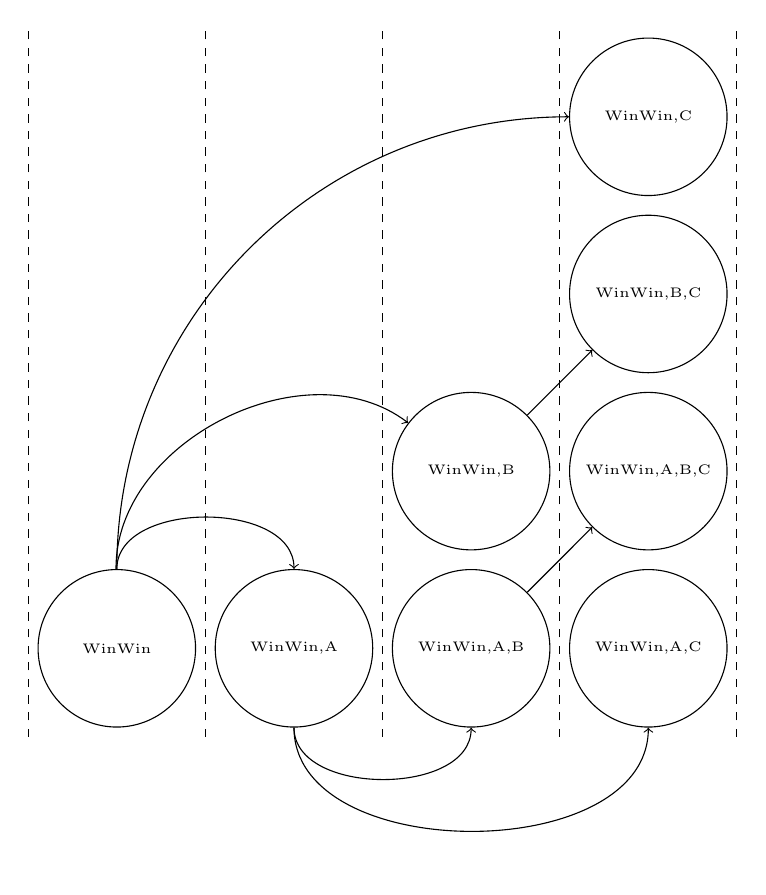
\begin{tikzpicture}[every node/.style={draw,circle, minimum size=2cm}, scale=0.75]
	\node at (0, 0) (W) 	{\tiny WinWin};
	\node at (3, 0) (WA)	{\tiny WinWin,A};
	\node at (6, 0) (WAB)	{\tiny WinWin,A,B};
	\node at (6, 3) (WB)	{\tiny WinWin,B};
	\node at (9, 3) (WABC)	{\tiny WinWin,A,B,C};
	\node at (9, 0) (WAC)	{\tiny WinWin,A,C};
	\node at (9, 6) (WBC)	{\tiny WinWin,B,C};
	\node at (9, 9) (WC)	{\tiny WinWin,C};

	\draw[dashed] (-1.5, -1.5) -- (-1.5, 10.5);
	\draw[dashed] (1.5, -1.5) -- (1.5, 10.5);
	\draw[dashed] (4.5, -1.5) -- (4.5, 10.5);
	\draw[dashed] (7.5, -1.5) -- (7.5, 10.5);
	\draw[dashed] (10.5, -1.5) -- (10.5, 10.5);

	\draw [->] (W) edge[bend left=90] (WA) (W) edge[bend left=64] (WB) (W) edge[bend left = 45] (WC);
	\draw [->] (WA) edge[bend right=90] (WAB) (WA) edge[bend right=90] (WAC);
	\draw [->] (WAB) edge (WABC);
	\draw [->] (WB) edge (WBC);
\end{tikzpicture}